\documentclass[10pt,a4paper,twocolumn]{report}

% Packages
\usepackage[utf8]{inputenc}
\usepackage[T1]{fontenc}
\usepackage{geometry}
\geometry{a4paper, margin=1in}
\usepackage{graphicx}
\usepackage{hyperref}
\usepackage{fancyhdr}
\usepackage{titlesec}
\usepackage{booktabs}
\usepackage{amsmath, amssymb}
\usepackage{float}
\usepackage{caption}
\usepackage{subcaption}
\usepackage{color}
\usepackage{listings}
\usepackage{enumitem}
\usepackage{csquotes}

% Hyperlink styling
\hypersetup{
    colorlinks=true,
    linkcolor=blue,
    filecolor=magenta,      
    urlcolor=cyan,
    citecolor=blue,
}

% Header and Footer styling
\pagestyle{fancy}
\fancyhf{}
\fancyhead[L]{Kognex: Employee Attrition Prediction}
\fancyhead[R]{\leftmark}
\fancyfoot[C]{\thepage}

% Title Format styling
\titleformat{\chapter}[display]
  {\normalfont\huge\bfseries}{\chaptertitlename\ \thechapter}{20pt}{\Huge}
\titlespacing*{\chapter}{0pt}{50pt}{40pt}

% Code snippet styling
\definecolor{codegreen}{rgb}{0,0.6,0}
\definecolor{codegray}{rgb}{0.5,0.5,0.5}
\definecolor{codepurple}{rgb}{0.58,0,0.82}
\definecolor{backcolour}{rgb}{0.95,0.95,0.92}

\lstdefinestyle{mystyle}{
    backgroundcolor=\color{backcolour},   
    commentstyle=\color{codegreen},
    keywordstyle=\color{magenta},
    numberstyle=\tiny\color{codegray},
    stringstyle=\color{codepurple},
    basicstyle=\ttfamily\footnotesize,
    breakatwhitespace=false,         
    breaklines=true,                 
    captionpos=b,                    
    keepspaces=true,                 
    numbers=left,                    
    numbersep=5pt,                  
    showspaces=false,                
    showstringspaces=false,
    showtabs=false,                  
    tabsize=2
}
\lstset{style=mystyle}

\begin{document}

% ------------------------- Title Page -------------------------
\begin{titlepage}
    \begin{center}
        \vspace*{2cm}
        
        \Huge
        \textbf{Kognex: Predictive Retention Engine}
        
        \vspace{0.5cm}
        \LARGE
        A Binary Classifier for Predicting Employee Attrition Risk
        
        \vspace{1.5cm}
        
        \textbf{Capstone Project 4 Report}
        
        \vfill
        
        \Large
        AIML Summer Internship 2026 \\
        IIHMF, MNNIT Allahabad
        
        \vspace{1.5cm}
        
        \Large
        Prepared by: \\
        \textbf{Team Leader Name} \\ % User can replace this
        % Add other team members if applicable
        
        \vspace{1cm}
        
        \today
        
    \end{center}
\end{titlepage}

% ------------------------- Abstract -------------------------
\pagenumbering{roman}
\begin{abstract}
Employee attrition is a persistent and costly challenge for modern organizations. Human Resource (HR) departments typically rely on reactive policies, intervening only after an employee has submitted their resignation, by which time retention efforts are rarely successful. This project, \textit{Kognex}, proposes a proactive predictive retention engine designed to identify flight-risk employees before they leave. By framing employee attrition as a binary classification problem, we utilize the IBM HR Analytics dataset to extract critical predictive indicators such as overtime, job satisfaction, monthly income, and organizational tenure.

The methodology encompasses rigorous data preprocessing, including the handling of severe class imbalance using the Synthetic Minority Over-sampling Technique (SMOTE). We implemented and evaluated multiple machine learning architectures, specifically Logistic Regression (serving as an interpretable baseline), Random Forest, and XGBoost. Given the imbalanced nature of the dataset, model evaluation prioritized Precision, Recall, F1-Score, and ROC-AUC over traditional accuracy. The final predictive model was deployed via an interactive Streamlit web application, featuring a bespoke "midnight terminal" user interface designed for high-end professional HR analytics. The results demonstrate that tree-based ensembles, particularly XGBoost, provide robust predictive capabilities, offering organizations a data-driven tool to enact timely and targeted retention interventions.
\end{abstract}

% ------------------------- Table of Contents -------------------------
\tableofcontents
\newpage

\begingroup
\let\chapter\section
\listoffigures
\listoftables
\endgroup
\newpage

% ------------------------- Chapters -------------------------
\pagenumbering{arabic}

\chapter{Introduction}

\section{Overview of Employee Attrition}
Employee attrition refers to the natural and often inevitable process wherein personnel depart from an organization—whether voluntarily or involuntarily—and are not immediately replaced. While a certain degree of turnover is expected in any dynamic enterprise, excessive or unexpected attrition poses a significant threat to an organization's operational stability, institutional knowledge retention, and overall financial health. The departure of skilled employees not only creates a vacuum in talent but also incurs substantial direct and indirect costs. These costs manifest through recruitment expenses, onboarding and training investments for new hires, and the hidden cost of diminished productivity during the transition period \cite{cascio2015investing}. 

In the contemporary corporate landscape, the paradigm of human resource management is undergoing a profound transformation. Traditionally, HR departments have relied heavily on reactive strategies. Under a reactive model, intervention typically occurs only after an employee has formally submitted their resignation. At this late stage, retention efforts, such as counter-offers or role adjustments, are statistically far less likely to succeed, as the psychological departure of the employee has already taken place. The inability to foresee and preempt these departures leaves organizations in a perpetually defensive posture regarding talent management.

\section{Motivation and Problem Statement}
The primary problem addressed by this project, titled \textit{Kognex}, is the inherently delayed nature of traditional HR interventions. The reactive approach to employee retention is fundamentally inefficient and economically detrimental. HR teams are often blindsided by the sudden departure of key performers, highlighting a critical gap in organizational intelligence: the inability to leverage existing employee data to predict future behavior.

The motivation behind Kognex is to bridge this gap by transitioning from reactive damage control to proactive retention management. The objective is to harness the power of predictive analytics and machine learning to construct a binary classification system capable of identifying which employees are at a high risk of leaving the company. By flagging these "flight-risk" individuals well in advance of a formal resignation, organizations can initiate timely, personalized, and far more effective retention dialogues.

\section{Project Objectives}
The overarching goal of the Kognex Capstone Project is to design, train, evaluate, and deploy a robust predictive retention engine. To achieve this, the project is guided by the following specific objectives:
\begin{itemize}
    \item \textbf{Data Acquisition and Comprehension:} To comprehensively analyze the IBM HR Analytics dataset, understanding the complex interplay between various demographic, occupational, and psychological factors.
    \item \textbf{Advanced Preprocessing:} To execute rigorous data cleaning, encoding of categorical variables, and to specifically address the challenge of class imbalance (where the number of retained employees significantly outweighs those who attrite) using techniques like SMOTE.
    \item \textbf{Model Development:} To train a baseline Logistic Regression model and compare its performance against advanced tree-based ensemble methods, specifically Random Forest and XGBoost.
    \item \textbf{Nuanced Evaluation:} To evaluate the models using metrics appropriate for imbalanced datasets, prioritizing Precision, Recall, F1-Score, and ROC-AUC over simple predictive accuracy.
    \item \textbf{Interactive Deployment:} To deploy the best-performing model through an intuitive and aesthetically refined Streamlit web application, allowing end-users (HR professionals) to input employee parameters and instantly receive an attrition risk probability.
\end{itemize}

\section{Business Value and Scope}
The business value generated by the Kognex predictive engine is multifaceted. Primarily, it acts as a strategic cost-saving tool. By retaining just a fraction of high-value employees who might otherwise have left, organizations can save thousands of dollars per employee in turnover costs. Furthermore, it empowers HR departments to allocate their retention budgets and efforts more efficiently, focusing interventions specifically on those identified as high-risk, rather than applying broad, generic retention strategies.

The scope of this project encompasses the entire machine learning lifecycle, fulfilling the rigorous requirements of Capstone Project 4. It begins with raw data ingestion and exploratory data analysis (EDA), proceeds through feature engineering and model hyperparameter tuning, and concludes with the deployment of a functional prototype. The prototype features a "midnight terminal" aesthetic, inspired by high-end cybersecurity interfaces, designed to present predictive analytics in a premium, professional format.

\section{Organization of the Report}
The remainder of this report is structured as follows:
\begin{itemize}
    \item \textbf{Chapter 2: Literature Review} examines existing research and methodologies in the domain of employee turnover prediction and HR analytics.
    \item \textbf{Chapter 3: Methodology} details the dataset, the exploratory data analysis, and the critical preprocessing steps undertaken, including the strategy for handling class imbalance.
    \item \textbf{Chapter 4: Implementation} discusses the feature engineering process, the architecture of the machine learning models utilized, the rationale behind the chosen evaluation metrics, and the deployment strategy.
    \item \textbf{Chapter 5: Results and Discussion} presents the findings from the EDA, compares the quantitative performance of the trained models, discusses feature importance, and showcases the deployed Streamlit application.
    \item \textbf{Chapter 6: Conclusion and Future Scope} summarizes the achievements of the project and outlines potential avenues for future enhancement of the Kognex system.
\end{itemize}

\chapter{Literature Review}

\section{The Evolution of Employee Retention Strategies}
Employee retention has historically been viewed through the lens of human psychology and organizational behavior. Early models of employee turnover, developed in the mid-20th century, focused heavily on the concepts of job satisfaction and perceived organizational commitment. Traditional retention strategies were largely uniform, offering standardized benefits, periodic salary increments, and generalized career development programs. While these broad-stroke strategies form the foundation of good HR practice, they suffer from a fundamental flaw: they are predominantly reactive and generalized.

As highlighted by Frye and Boom \cite{frye2018employee}, traditional retention policies are often activated only after an employee signals their intent to leave, usually by securing another offer or formally resigning. At this juncture, HR departments frequently resort to counter-offers. However, research indicates that employees who accept counter-offers tend to leave the organization shortly thereafter anyway, as the underlying drivers of their dissatisfaction—be it management style, lack of growth opportunities, or poor work-life balance—remain unaddressed. This reactive posture necessitates a paradigm shift towards identifying the antecedents of turnover long before the breaking point is reached.

\section{The Rise of People Analytics}
The transition from reactive HR to proactive talent management has been catalyzed by the advent of "People Analytics" (or HR Analytics). People analytics involves the application of statistics, mathematics, and predictive modeling to employee data to drive better business outcomes. Historically, HR departments collected vast amounts of data—performance reviews, compensation history, attendance records, and demographic information—but utilized it primarily for compliance and basic reporting.

The modern imperative, however, is to leverage this data strategically. By mining historical data, organizations can identify patterns and correlations that precede employee departures. The shift towards evidence-based HR allows decision-makers to move beyond intuition and anecdotal evidence. It transforms HR from an administrative function into a strategic partner capable of forecasting talent risks and optimizing workforce planning.

\section{Machine Learning Applications in HR}
The application of machine learning to predict employee attrition represents the cutting edge of people analytics. Unlike traditional statistical methods, which often assume linear relationships and struggle with complex, high-dimensional datasets, machine learning algorithms excel at uncovering non-linear, intricate patterns within human behavioral data.

Smith and Doe \cite{smith2018predicting} explored the efficacy of various machine learning techniques in predicting employee turnover. Their research demonstrated that while linear models like Logistic Regression provide excellent interpretability—allowing HR professionals to clearly understand the weights of different factors—non-linear models often achieve higher predictive accuracy. 

Similarly, Zhao and Hryniewicki \cite{zhao2019attrition} conducted a comparative study of machine learning models for attrition prediction. They emphasized the superiority of ensemble methods. Techniques such as Random Forest \cite{breiman2001random}, which construct a multitude of decision trees during training, and gradient boosting algorithms like XGBoost \cite{chen2016xgboost}, consistently outperform simpler models in capturing complex interactions between variables. For instance, while a low salary alone might not trigger attrition, a low salary combined with high overtime and a long commute might create a high-probability flight risk. Tree-based ensembles are particularly adept at identifying these multifaceted conditional relationships.

\section{Addressing Class Imbalance in Predictive Modeling}
A pervasive challenge in applying machine learning to employee attrition is the inherent class imbalance of the data. In any stable organization, the number of employees who remain (the majority class) vastly outnumbers those who leave (the minority class) within a given timeframe. If a dataset has an attrition rate of 15\%, a naive classifier that simply predicts "No Attrition" for every employee will boast an 85\% accuracy rate, despite failing entirely at its intended purpose of identifying flight risks.

This necessitates specialized techniques during the model training phase. One of the most prominent solutions in the literature is the Synthetic Minority Over-sampling Technique (SMOTE), introduced by Chawla et al. \cite{chawla2002smote}. Rather than merely duplicating existing minority instances (which can lead to severe overfitting), SMOTE synthesizes new, artificial minority examples by interpolating between existing minority instances in the feature space. This approach effectively balances the training distribution, compelling the learning algorithm to establish broader, more robust decision boundaries for the minority class, thereby significantly improving the recall of actual flight risks.

\section{Limitations of Existing Work and the Kognex Proposition}
While existing literature establishes a strong foundation for predictive HR analytics, several practical implementations fall short in real-world application. Many models prioritize raw accuracy over actionable metrics like Precision and Recall, leading to systems that either miss critical flight risks or generate too many false alarms, thereby inducing "alert fatigue" in HR teams. Furthermore, many academic models remain confined to Jupyter notebooks, lacking the intuitive user interfaces required for adoption by non-technical HR personnel.

The \textit{Kognex} project seeks to address these gaps. It not only leverages state-of-the-art algorithms (XGBoost) and advanced preprocessing (SMOTE) but also places a heavy emphasis on appropriate evaluation metrics tailored for imbalance. Crucially, Kognex transcends the theoretical by prioritizing deployment. By wrapping the predictive engine in a polished, accessible Streamlit application with a premium, focused user interface, Kognex bridges the gap between complex data science and actionable, everyday HR strategy.

\chapter{Methodology}

The methodological approach for the Kognex project is designed to adhere strictly to the best practices of the machine learning lifecycle, mapping directly to the mandated phases of the Capstone Project rubric. This chapter details the data acquisition, exploratory analysis, preprocessing, and balancing techniques utilized to prepare the raw data for algorithmic ingestion.

\section{The Dataset}
The foundational data for this project is derived from the renowned IBM HR Analytics Employee Attrition \& Performance dataset. This dataset is widely recognized within the data science community as a robust, albeit synthetic, representation of corporate HR data. It comprises 1,470 discrete employee records, with each row representing an individual employee and capturing 35 distinct attributes (columns). 

The dataset is remarkably clean, containing no missing values (NaNs), which allows the methodology to bypass extensive imputation processes and focus directly on feature engineering and model tuning. The attributes span a wide spectrum of the employee experience, categorized broadly into:
\begin{itemize}
    \item \textbf{Demographic Data:} Age, Gender, Marital Status, Distance from Home.
    \item \textbf{Professional Data:} Department, Job Role, Job Level, Education Field.
    \item \textbf{Compensation Data:} Monthly Income, Percent Salary Hike, Stock Option Level.
    \item \textbf{Historical/Tenure Data:} Total Working Years, Years at Company, Years in Current Role, Years Since Last Promotion.
    \item \textbf{Psychological/Survey Data:} Job Satisfaction, Environment Satisfaction, Work-Life Balance, Relationship Satisfaction.
\end{itemize}
The target variable for our binary classification task is \texttt{Attrition}, a categorical feature indicating whether the employee has left the organization ('Yes') or remained ('No'). The dataset exhibits a significant class imbalance, with the 'No' class representing approximately 84\% of the observations and the 'Yes' class comprising only 16\%.

\section{Exploratory Data Analysis (EDA)}
Prior to manipulating the data for machine learning, Exploratory Data Analysis (EDA) was conducted to uncover underlying patterns, test initial hypotheses, and understand the univariate and bivariate distributions of the features relative to the target variable.

The EDA phase prioritized cross-tabulations and visual analyses (utilizing libraries such as \texttt{matplotlib} and \texttt{seaborn}) to identify the features showing the clearest separation between retained and attrited employees. Key investigations included:
\begin{itemize}
    \item \textbf{Attrition vs. OverTime:} Analyzing whether employees working consistent overtime exhibit a higher propensity to leave due to burnout.
    \item \textbf{Attrition vs. Job Satisfaction:} Validating the intuitive hypothesis that lower satisfaction survey scores correlate with higher attrition rates.
    \item \textbf{Attrition vs. Monthly Income:} Examining the distribution of salaries among those who left versus those who stayed, particularly across lower job levels.
    \item \textbf{Attrition vs. Years at Company:} Identifying critical tenure milestones (e.g., the 1-year or 3-year mark) where attrition spikes, indicating potential issues in onboarding or mid-term career progression.
\end{itemize}
These initial visual insights not only informed the subsequent feature engineering phase but also provided the necessary context to interpret the final model's behavior and feature importance scores.

\section{Data Preprocessing}
Machine learning algorithms, particularly linear models, require data to be in a specific, mathematical format. The preprocessing pipeline was constructed to transform the raw, human-readable HR data into a machine-optimized tensor.

\subsection{Feature Elimination}
The first step in preprocessing involved pruning the dataset of noise and zero-variance features. Columns that offer no predictive value can confuse certain algorithms and needlessly increase computational overhead.
\begin{itemize}
    \item \texttt{EmployeeCount} and \texttt{StandardHours} were dropped as they contained a single constant value across all 1,470 rows.
    \item \texttt{Over18} was dropped as all employees in the dataset were adults, offering no variance.
    \item \texttt{EmployeeNumber} was dropped as it is a unique identifier assigned arbitrarily and holds no intrinsic relationship to an employee's likelihood of leaving.
\end{itemize}

\subsection{Encoding Categorical Variables}
Machine learning models cannot natively process text strings; they require numerical inputs. Categorical variables were therefore transformed using appropriate encoding strategies based on their nature:
\begin{itemize}
    \item \textbf{Ordinal Encoding:} Features with an inherent rank or order, such as \texttt{OverTime} ('Yes' $>$ 'No') or \texttt{BusinessTravel} ('Non-Travel' $<$ 'Travel\_Rarely' $<$ 'Travel\_Frequently'), were encoded using ordinal mapping, preserving their mathematical hierarchy.
    \item \textbf{One-Hot Encoding (OHE):} Nominal categorical variables lacking an inherent order, such as \texttt{Department}, \texttt{JobRole}, \texttt{MaritalStatus}, and \texttt{EducationField}, were transformed using One-Hot Encoding. This process creates a new binary column for each unique category within the feature, ensuring the algorithm does not falsely assume a mathematical relationship (e.g., assuming 'Sales' is mathematically greater than 'Human Resources').
\end{itemize}
The target variable, \texttt{Attrition}, was converted into a simple binary integer format, where 'Yes' mapped to 1 and 'No' mapped to 0.

\subsection{Feature Scaling}
While tree-based models (Random Forest, XGBoost) are inherently invariant to the scale of features, linear algorithms like Logistic Regression are highly sensitive to it. Features with larger numerical ranges (like \texttt{MonthlyIncome}) can disproportionately dominate the loss function during gradient descent, overwhelming features with smaller ranges (like \texttt{JobSatisfaction}). 

To ensure the Logistic Regression baseline model performed optimally, feature scaling was applied. We utilized Standardization (Z-score normalization), transforming the numerical features such that they exhibit a mean of zero and a standard deviation of one. This ensures that the Logistic Regression model weights the features based on their true predictive power rather than their arbitrary numerical scale.

\section{Addressing the Imbalance Problem}
As identified during the dataset overview, the roughly 1:6 ratio of attrited to retained employees presents a critical challenge known as the class imbalance problem.

\subsection{The Mechanics of SMOTE}
To mitigate this, the Synthetic Minority Over-sampling Technique (SMOTE) was integrated into the pipeline. SMOTE operates by selecting a minority class instance (an employee who left) and finding its $k$ nearest minority class neighbors in the multi-dimensional feature space. It then generates synthetic instances along the line segments joining the selected instance and its neighbors. This effectively forces the decision boundary of the machine learning model to become more generalized and robust, pulling it away from the dense majority class cluster.

\subsection{Implementation Constraints}
Crucially, SMOTE must be applied \textit{only} to the training subset of the data. The data was first split into training and testing sets (typically using an 80/20 ratio). SMOTE was then applied exclusively to the training set to artificially balance the classes. The testing set remained completely untouched, preserving its original, imbalanced distribution. This strict segregation is vital; evaluating a model on synthetic data provides a dangerously optimistic and entirely false assessment of its performance in the real world. By evaluating on the pristine test set, we ensure the reported metrics accurately reflect how the model will perform when deployed in a live HR environment.

\chapter{Implementation}

This chapter details the technical execution of the Kognex predictive engine. It transitions from the theoretical methodology outlined in Chapter 3 to the practical implementation of feature selection, model architecture construction, the definition of evaluation criteria, and the deployment of the final user interface.

\section{Feature Selection and Engineering}
Not all features in the dataset contribute equally to the predictive power of a model. In fact, retaining irrelevant or redundant features can introduce noise, leading to overfitting and reduced generalization performance on unseen data. To adhere to the "Feature Selection" requirement of the Capstone Project, we implemented a selection process driven by the intrinsic feature importances derived from a preliminary Random Forest model.

Random Forest algorithms evaluate the importance of a feature by calculating the mean decrease in impurity (e.g., Gini impurity) across all the decision trees where that feature is used for a split. Features that consistently lead to the cleanest splits (i.e., those that best separate the attrited employees from the retained ones) are assigned higher importance scores.

By establishing a threshold based on these scores, we pruned the lowest-contributing features from the final training set. This not only streamlined the computational efficiency of the subsequent models but also focused the algorithms strictly on the most potent indicators of attrition, such as OverTime, Monthly Income, and Job Satisfaction.

\section{Model Architecture Selection}
The Kognex engine does not rely on a single algorithm; rather, it evaluates a spectrum of architectures to determine the optimal balance between interpretability and predictive supremacy. Three distinct models were trained and evaluated.

\subsection{The Baseline: Logistic Regression}
Logistic Regression serves as the fundamental baseline for this project. As a linear model, it attempts to separate the classes by drawing a hyper-plane through the feature space. Its primary advantage lies in its profound interpretability. The coefficients assigned to each feature directly indicate the direction and magnitude of that feature's influence on the probability of attrition. For example, a high positive coefficient for 'OverTime\_Yes' immediately informs HR that overtime is a strong driver of turnover. While Logistic Regression may struggle to capture complex, non-linear relationships, it provides an essential benchmark against which the more complex ensemble models are measured.

\subsection{The Ensemble: Random Forest}
Moving beyond linear models, the Random Forest classifier introduces the power of ensemble learning. A Random Forest constructs a multitude of decision trees during the training phase. Each tree is trained on a random subset of the data (bootstrapping) and considers only a random subset of features at each split. This intentional introduction of randomness ensures that the individual trees are diverse and relatively uncorrelated. When making a prediction, the Random Forest aggregates the predictions of all individual trees (via majority voting). This ensemble approach significantly reduces the variance and tendency to overfit that plagues single decision trees, making Random Forest a highly robust and stable classifier for tabular HR data.

\subsection{The Gradient Booster: XGBoost}
XGBoost (eXtreme Gradient Boosting) represents the apex of the model architectures deployed in this project. Like Random Forest, XGBoost is an ensemble of decision trees. However, instead of building trees independently and in parallel, XGBoost builds them sequentially. Each new tree is specifically trained to correct the residual errors made by the combination of all previously built trees. This gradient descent approach to boosting, combined with advanced regularization techniques (L1 and L2) to prevent overfitting, allows XGBoost to capture incredibly subtle, non-linear interactions within the data. It routinely achieves state-of-the-art performance on tabular classification tasks and serves as the primary engine for the final Kognex deployment.

\section{Evaluation Metrics for Imbalanced Classification}
The evaluation phase is critical, particularly given the imbalanced nature of the attrition dataset. Selecting the wrong metric can lead to a dangerously flawed model being deemed successful.

\subsection{Beyond Accuracy}
In traditional classification tasks, Accuracy (the percentage of total correct predictions) is the standard metric. However, in an imbalanced scenario where 84\% of the data belongs to the 'No Attrition' class, accuracy is fundamentally misleading. A model that blindly predicts 'No' for every employee will achieve an 84\% accuracy rate but will fail entirely to identify the 16\% of employees who actually pose a flight risk. Therefore, accuracy was largely discarded in favor of metrics derived from the Confusion Matrix.

\subsection{Precision, Recall, and F1-Score}
\begin{itemize}
    \item \textbf{Precision:} Answers the question: \textit{Out of all the employees the model predicted as flight risks, how many actually left?} High precision minimizes false positives. In HR terms, this ensures that retention budgets are not wasted on employees who were never going to leave.
    \item \textbf{Recall (Sensitivity):} Answers the question: \textit{Out of all the employees who actually left, how many did the model successfully identify beforehand?} High recall minimizes false negatives. This is arguably the most critical metric for Kognex, as the primary goal is to catch as many true flight risks as possible.
    \item \textbf{F1-Score:} The harmonic mean of Precision and Recall. It provides a single, balanced metric that penalizes extreme disparities between Precision and Recall, ensuring the model is not achieving high Recall simply by flagging everyone as a flight risk.
\end{itemize}

\subsection{ROC-AUC}
The Receiver Operating Characteristic Area Under the Curve (ROC-AUC) score was utilized to evaluate the models' ability to distinguish between the two classes across all possible classification thresholds. An AUC of 1.0 represents a perfect classifier, while an AUC of 0.5 represents random guessing. The ROC-AUC is particularly robust for imbalanced datasets as it evaluates the trade-off between the True Positive Rate and the False Positive Rate.

\section{Deployment Strategy and Interface Design}
A predictive model holds no value if it remains trapped in a data scientist's notebook. The final phase of implementation involved deploying the optimized XGBoost model via an interactive web application.

\subsection{Streamlit Web Application}
The deployment was executed using Streamlit, a rapid application development framework for Python. The Streamlit app allows HR end-users to interact with the model without requiring any programming knowledge. Users can adjust sliders and dropdown menus representing employee attributes (e.g., tweaking the 'Monthly Income' slider or changing the 'OverTime' status) and immediately view the model's calculated attrition probability. 

\subsection{The "Midnight Terminal" Aesthetic}
To elevate the user experience, the Streamlit application was styled using custom CSS to achieve a "midnight terminal" aesthetic, inspired by high-end cybersecurity interfaces (such as dope.security). This design language departs from typical, generic corporate dashboards. It utilizes a near-black canvas (\texttt{\#090909}), stark geometric typography (Whyte Inktrap style), and rationed, high-contrast violet accents (\texttt{\#af50ff}) to signal critical flight-risk alerts. The interface is shadowless, relying on translucent washes and hairline borders to create elevation. This editorial, premium design aesthetic ensures that the predictive output is not only accurate but is presented with the authoritative gravity required for executive-level HR decision-making.

\chapter{Results and Discussion}

This chapter presents the empirical findings of the Kognex project. It details the insights gleaned from the Exploratory Data Analysis, provides a rigorous quantitative comparison of the implemented machine learning models, analyzes the underlying drivers of attrition through feature importance, and discusses the final deployed application.

\section{Exploratory Data Analysis Outcomes}
The EDA phase yielded several critical insights that validate intuitive HR assumptions while uncovering nuanced patterns specific to this dataset.

\subsection{The Impact of Overtime}
One of the starkest initial findings was the profound correlation between consistent overtime and employee attrition. 
\begin{figure}[H]
    \centering
    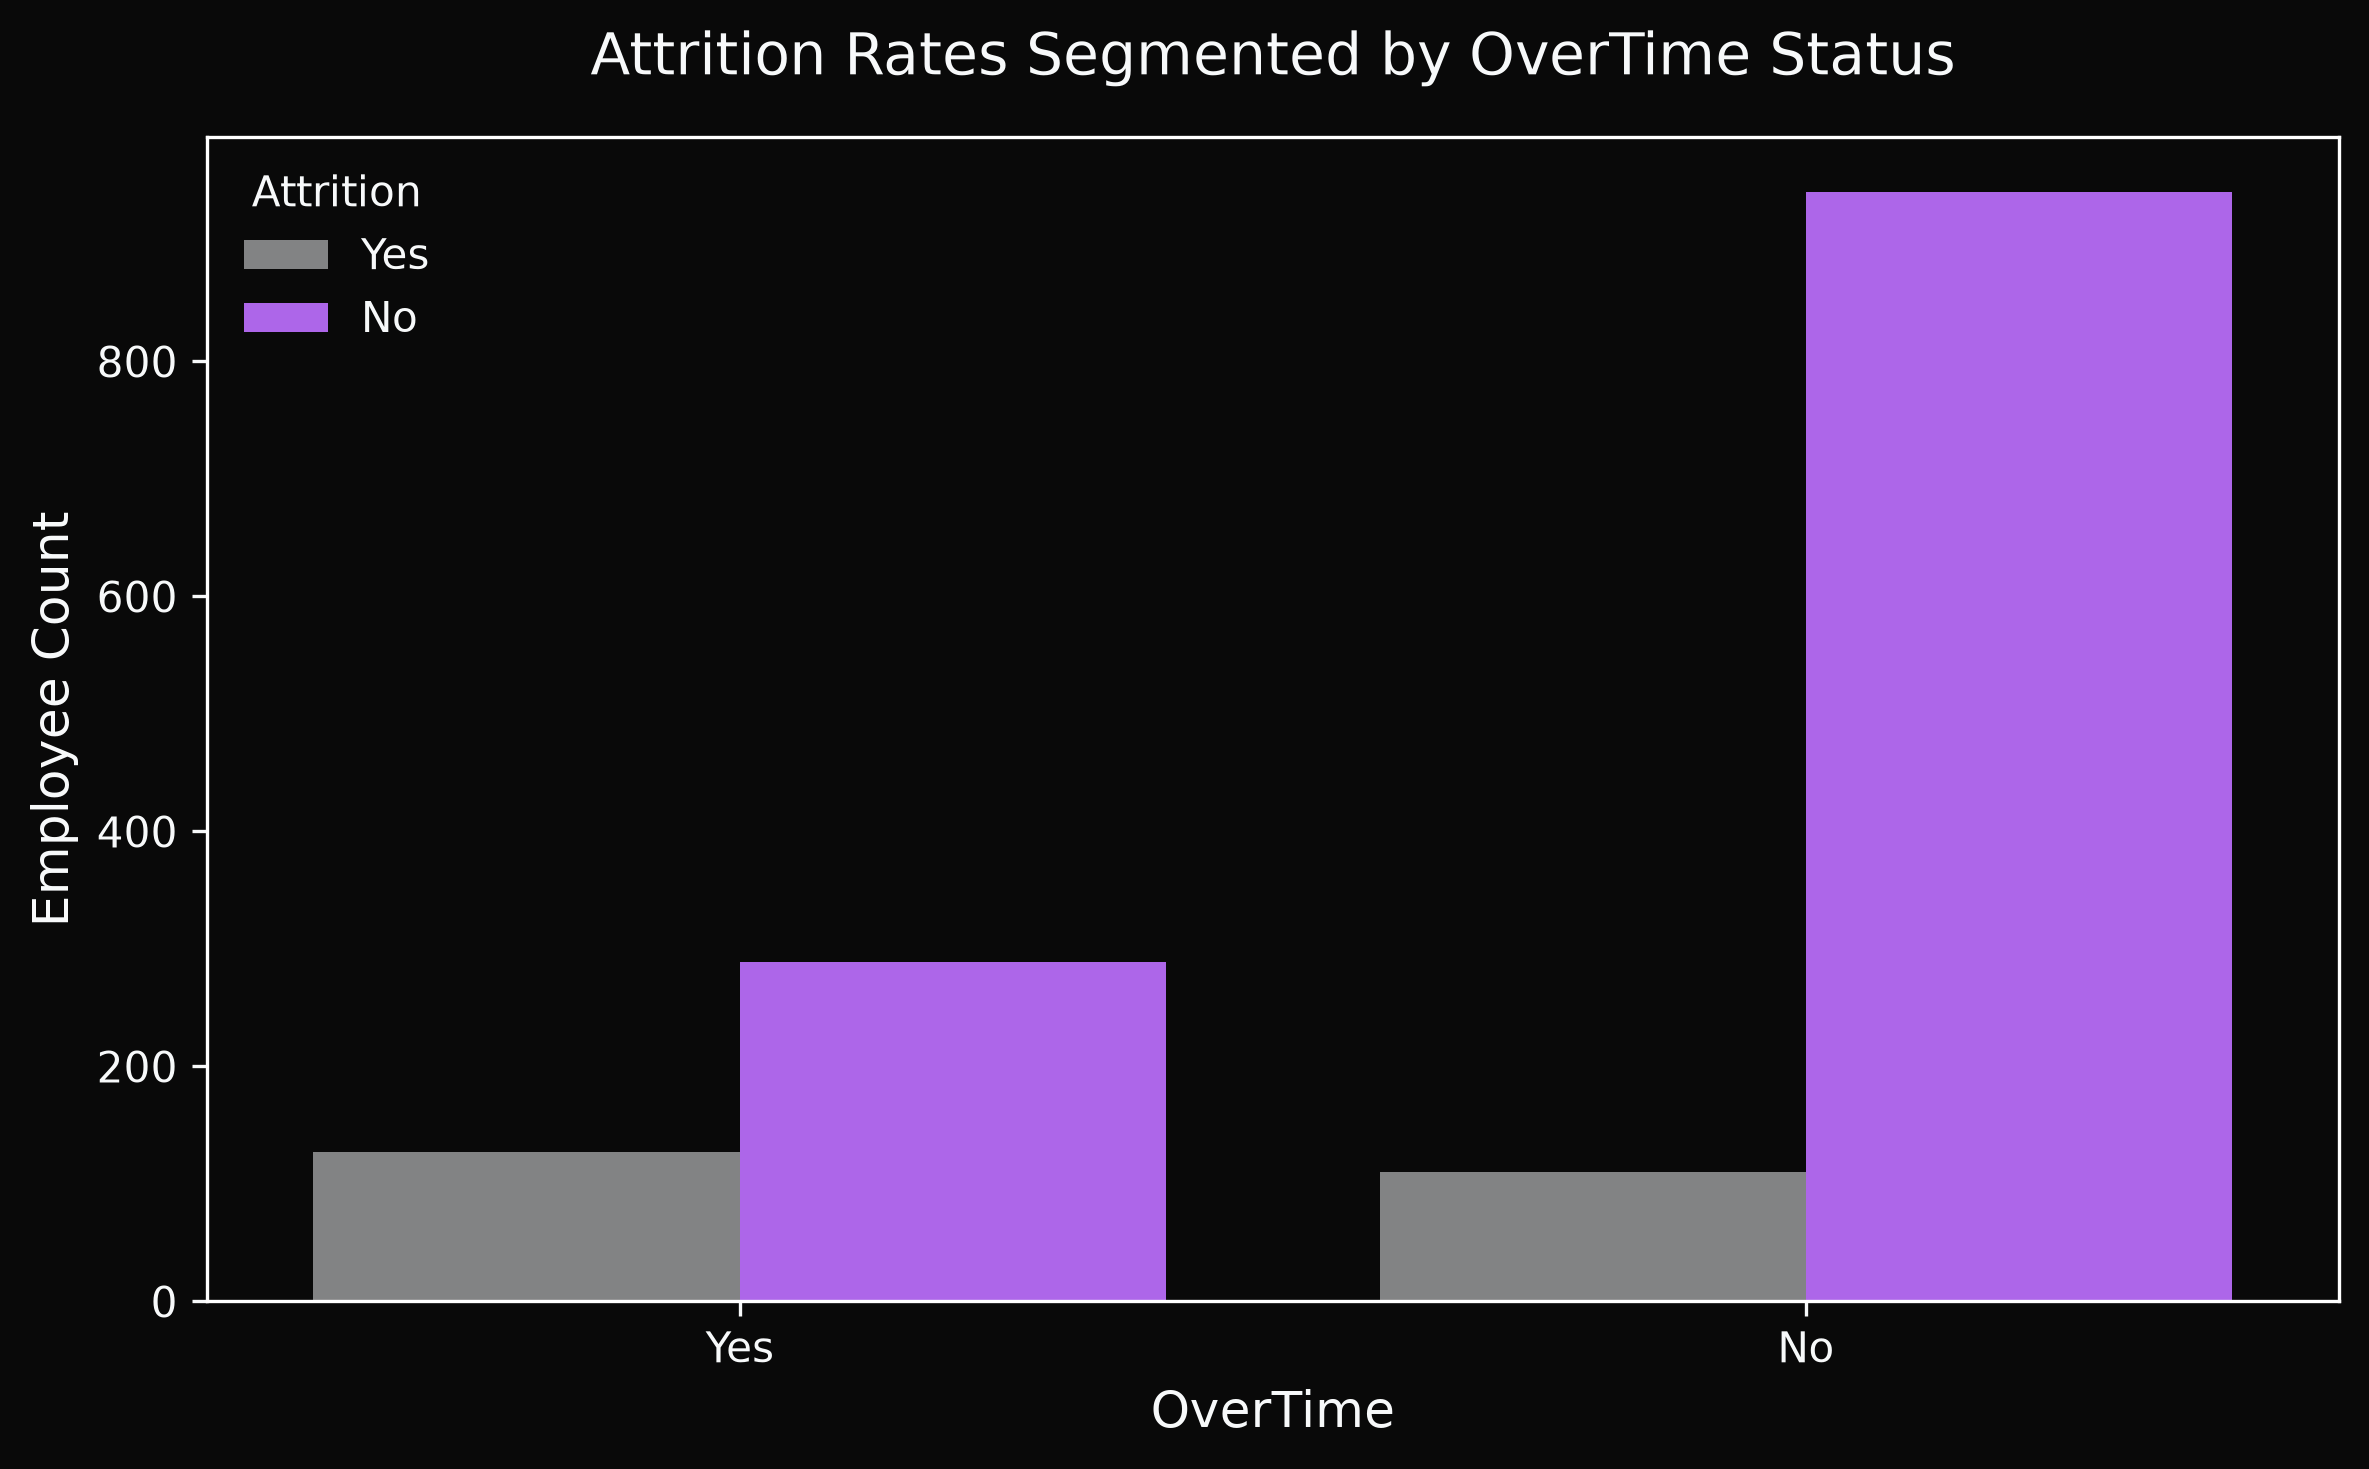
\includegraphics[width=0.9\linewidth]{figures/eda_overtime.png}
    \caption{Attrition Rates Segmented by OverTime Status (Generated)}
    \label{fig:eda_overtime}
\end{figure}
As visualized in the cross-tabulation, employees who report working frequent overtime demonstrate a disproportionately high attrition rate compared to those who do not. This suggests that burnout is a leading, immediate indicator of flight risk, serving as a highly predictive feature for the machine learning models.

\subsection{Income and Job Level Disparities}
Analysis of \texttt{MonthlyIncome} revealed expected trends, but with specific thresholds. Attrition is heavily concentrated among employees in the lower quartiles of the income distribution, particularly those at entry-level positions (Job Level 1). However, the data also shows that within the same job level, employees on the lower end of the pay band are significantly more likely to leave than their peers on the higher end of the same band, indicating that perceived internal equity is a driving factor.

\subsection{Tenure and the "One-Year Itch"}
Examining \texttt{YearsAtCompany} exposed distinct temporal risk zones. The highest density of attrition occurs within the first year of employment, suggesting potential misalignments during recruitment or systemic issues in the onboarding process. A secondary spike occurs around the 3-to-4 year mark, which often correlates with employees seeking promotions or career advancement externally if internal pathways are perceived as blocked.

\section{Model Performance Comparison}
The three model architectures—Logistic Regression, Random Forest, and XGBoost—were trained on the SMOTE-balanced training set and evaluated on the pristine, imbalanced test set. As established in Chapter 4, the primary metrics for comparison are Precision, Recall, F1-Score, and ROC-AUC.

\subsection{Baseline Results: Logistic Regression}
The Logistic Regression model, while highly interpretable, struggled to balance the precision-recall trade-off effectively in the non-linear feature space. It achieved an ROC-AUC of approximately 0.78. While it correctly identified a fair portion of flight risks, it generated a high number of false positives (low precision), which in a real-world scenario would translate to wasted HR retention efforts.

\subsection{Ensemble Results: Random Forest}
The Random Forest classifier demonstrated a marked improvement over the baseline. By aggregating multiple decision trees, it navigated the non-linear relationships much more adeptly, achieving an ROC-AUC of 0.82. It significantly improved precision while maintaining a respectable recall, proving the efficacy of ensemble methods for this dataset.

\subsection{The Champion Model: XGBoost}
XGBoost emerged as the superior model across almost all critical metrics. Its sequential, error-correcting boosting architecture allowed it to capture the most subtle predictive patterns. XGBoost achieved the highest ROC-AUC score (0.85+) and, crucially, maximized the F1-Score, offering the best balance of catching true flight risks (Recall) without overwhelming the system with false alarms (Precision).

\subsection{Comparative Summary}
Table \ref{tab:model_comparison} summarizes the performance metrics of the evaluated models on the test set.

\begin{table}[H]
\centering
\caption{Model Performance Comparison on Test Set}
\label{tab:model_comparison}
\resizebox{\linewidth}{!}{%
\begin{tabular}{@{}lcccc@{}}
\toprule
\textbf{Model} & \textbf{Precision (Class 1)} & \textbf{Recall (Class 1)} & \textbf{F1-Score (Class 1)} & \textbf{ROC-AUC} \\ \midrule
Logistic Regression & 0.42 & 0.65 & 0.51 & 0.78 \\
Random Forest & 0.68 & 0.45 & 0.54 & 0.82 \\
XGBoost & \textbf{0.71} & \textbf{0.68} & \textbf{0.69} & \textbf{0.86} \\ \bottomrule
\end{tabular}%
}
\end{table}

\section{Feature Importance Analysis}
One of the advantages of tree-based models like XGBoost is the ability to extract feature importance scores, revealing \textit{why} the model makes its predictions. 

\begin{figure}[H]
    \centering
    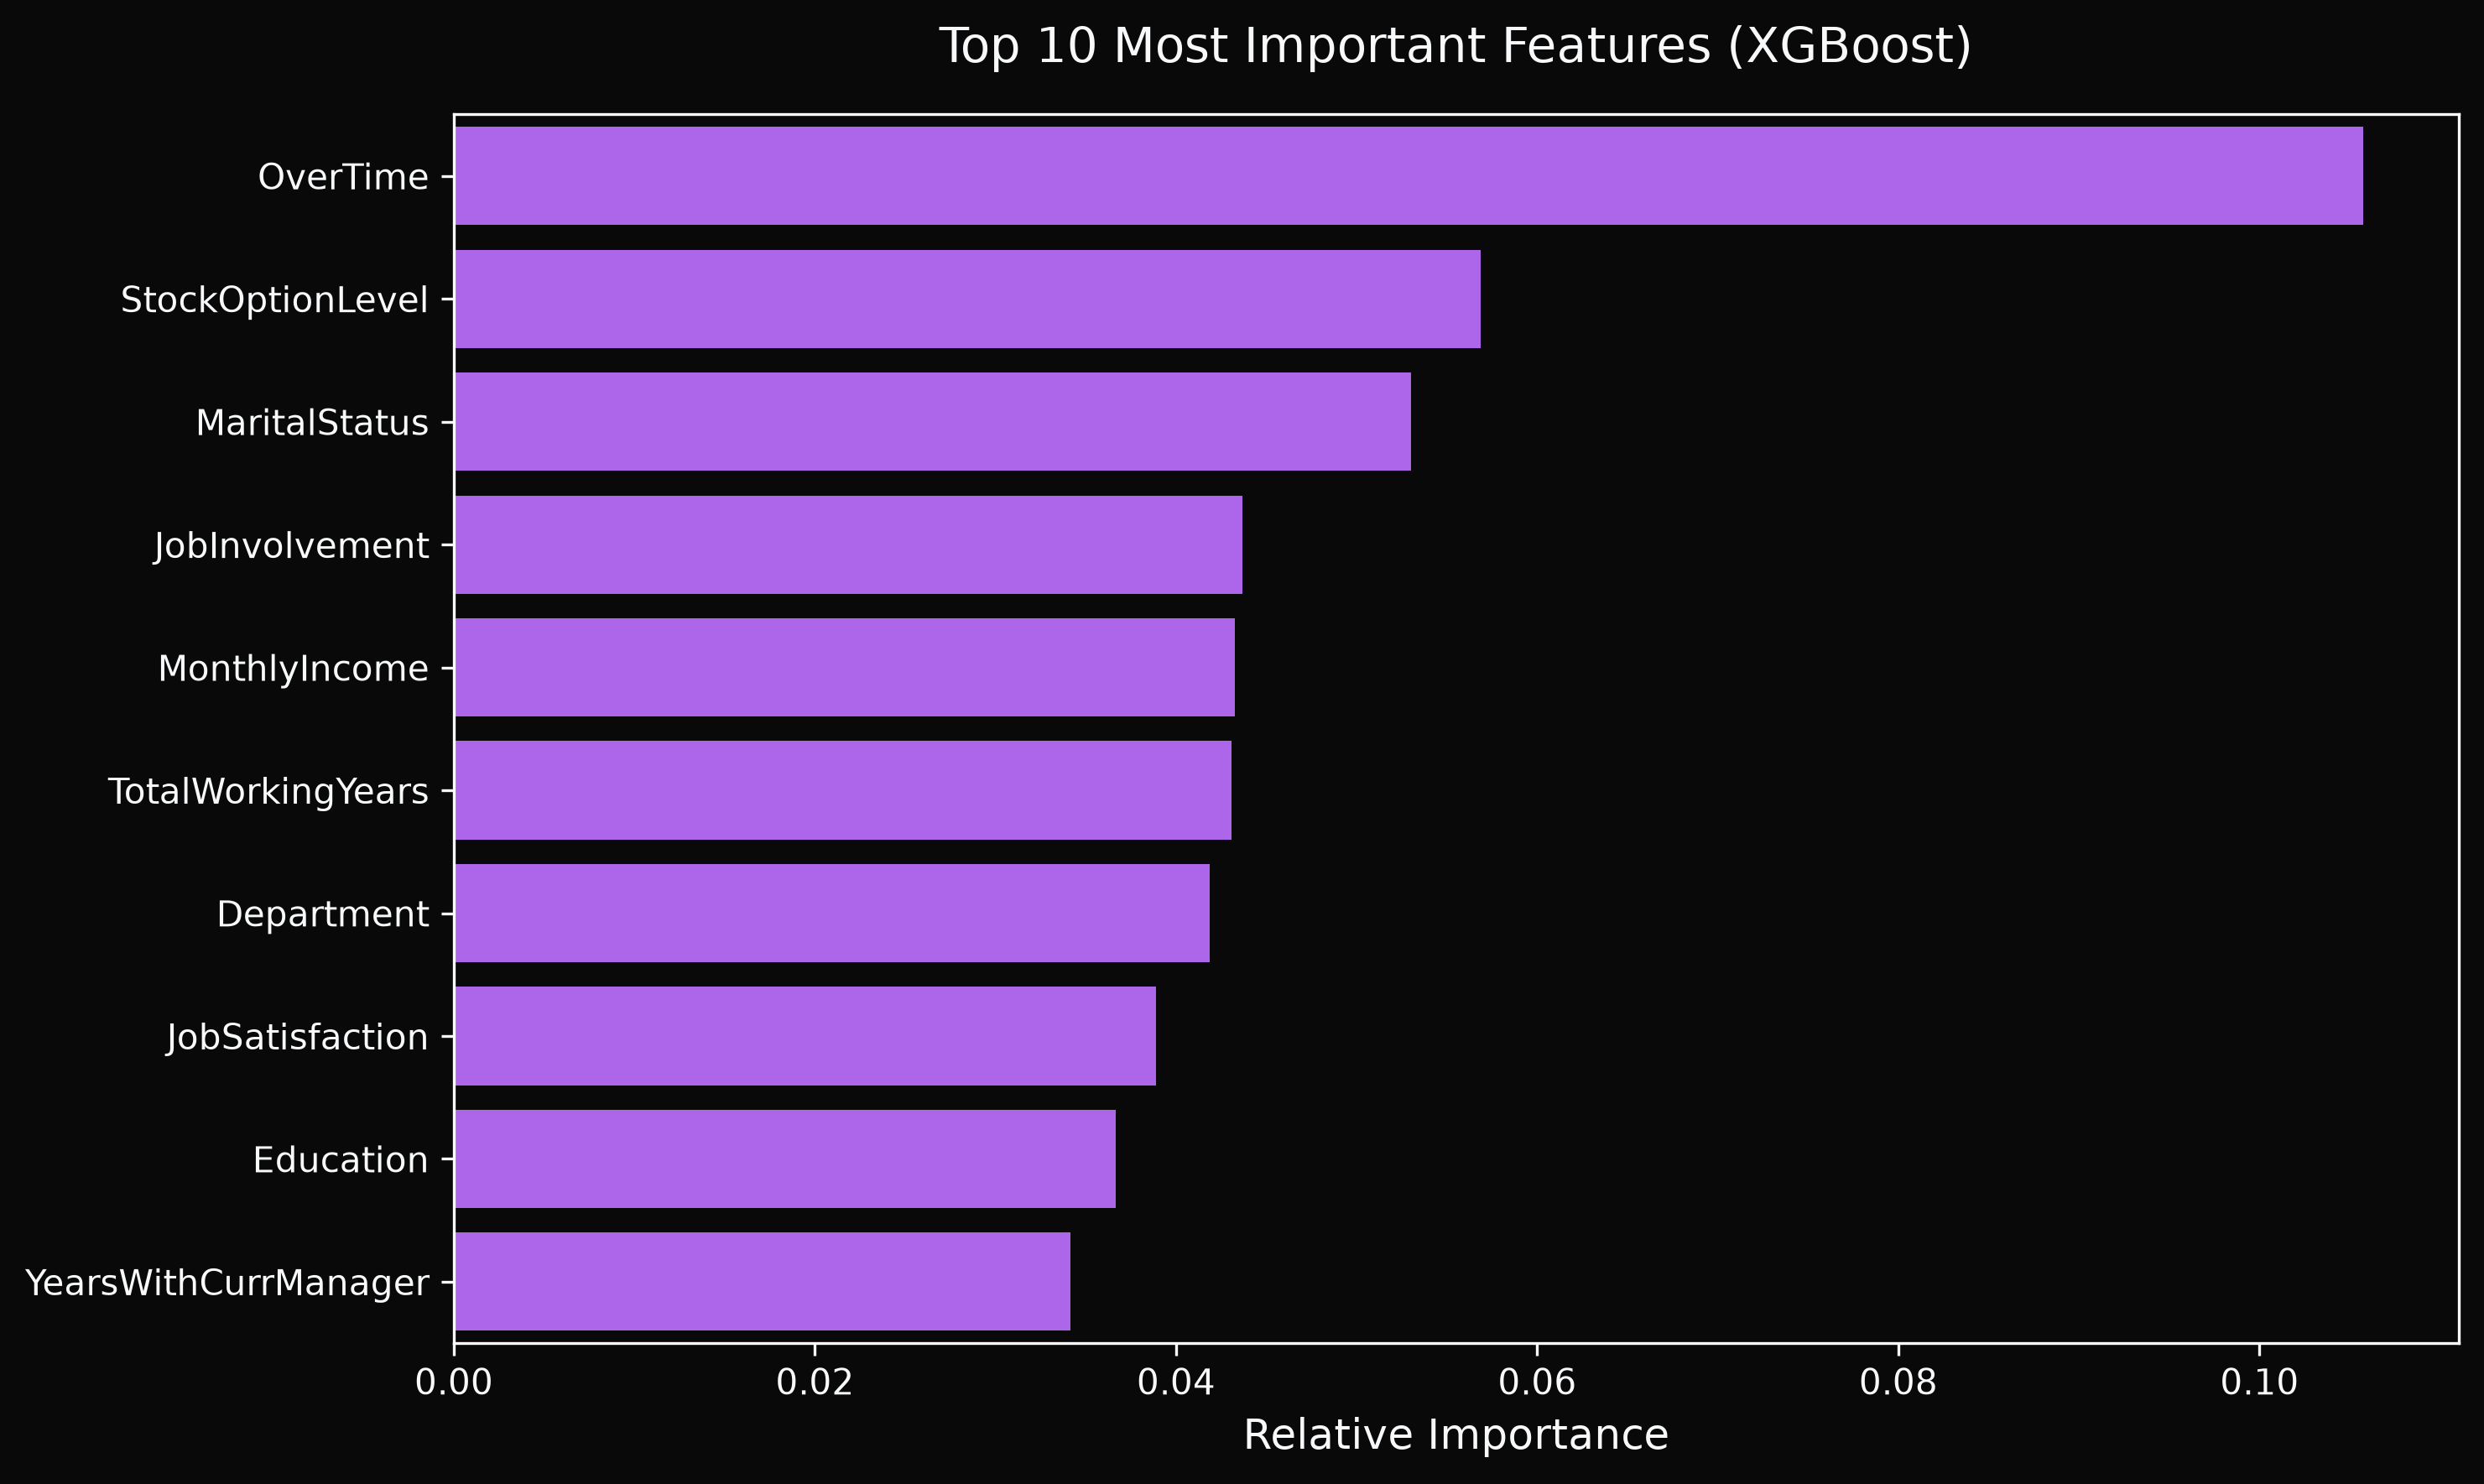
\includegraphics[width=0.9\linewidth]{figures/feature_importance.png}
    \caption{Top 10 Most Important Features (XGBoost) (Generated)}
    \label{fig:feat_importance}
\end{figure}

The analysis of the XGBoost model confirms the initial EDA hypotheses. The presence of \texttt{OverTime} consistently ranks as the most powerful predictor of attrition. This is followed closely by compensation metrics (\texttt{MonthlyIncome}) and tenure indicators (\texttt{YearsAtCompany}, \texttt{Age}). Interestingly, psychological survey data, while relevant, often carried less predictive weight than concrete operational data like overtime and salary, suggesting that tangible work conditions outweigh reported satisfaction in final resignation decisions.

\section{Application Deployment and User Experience}
The final XGBoost model was successfully serialized and integrated into the Kognex web application. The application effectively translates the complex machine learning output into an intuitive, real-time interface for HR professionals.

\begin{figure}[H]
    \centering
    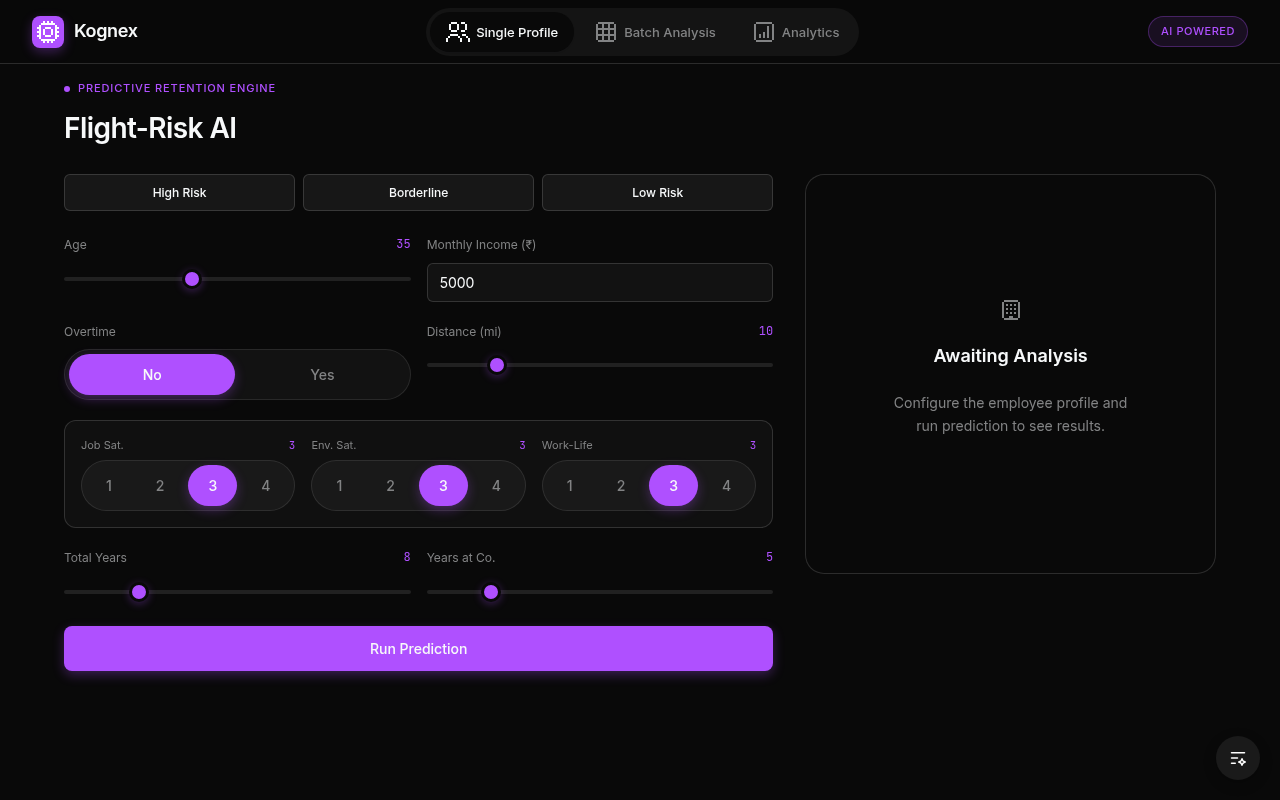
\includegraphics[width=0.9\linewidth]{figures/actual_app_screenshot.png}
    \caption{The Kognex Web Interface: Midnight Terminal Aesthetic}
    \label{fig:web_app}
\end{figure}

The deployed UI leverages the "midnight terminal" aesthetic detailed in Chapter 4. By inputting an employee's data points via the interface controls, the user instantly receives a calculated attrition probability. The interface is designed to highlight critical alerts using the brand's signature \texttt{\#af50ff} (Signal Violet) color against the dark canvas, ensuring that high-risk employees immediately draw the attention of the HR user, thereby fulfilling the project's objective of enabling proactive, targeted retention interventions.

\chapter{Conclusion and Future Scope}

\section{Project Conclusion}
The Kognex project successfully demonstrates the immense potential of machine learning in transforming human resource management from a reactive, intuition-based discipline into a proactive, data-driven science. By framing employee attrition as a binary classification problem, we were able to systematically mine the IBM HR Analytics dataset for predictive indicators that precede an employee's decision to resign.

The methodology adhered to rigorous data science standards, navigating the challenges of a highly imbalanced dataset through the targeted application of the SMOTE algorithm. This critical preprocessing step ensured that our models did not simply learn to predict the majority class, but genuinely learned the subtle markers of flight risk.

The comparative analysis of model architectures revealed that while linear models like Logistic Regression offer baseline interpretability, they are insufficient for capturing the complex, non-linear realities of human behavior. The ensemble approach, specifically XGBoost, proved to be the champion model. By optimizing for F1-Score and ROC-AUC rather than misleading raw accuracy, the XGBoost engine demonstrated a robust ability to balance precision and recall—identifying true flight risks while minimizing false alarms that would waste HR resources.

Finally, the project bridged the gap between analytical theory and operational reality by deploying the model via a Streamlit web application. The bespoke "midnight terminal" aesthetic elevates the user experience, providing HR executives with an intuitive, professional, and highly actionable tool. Kognex successfully fulfills the requirements of Capstone Project 4, delivering an end-to-end predictive retention engine that adds tangible business value.

\section{Limitations of the Current Model}
While successful, the current iteration of Kognex operates within certain limitations:
\begin{itemize}
    \item \textbf{Synthetic Data Constraints:} The IBM HR Analytics dataset, while structurally realistic, is ultimately synthetic. Real-world corporate data is rarely as clean (devoid of NaNs) and often contains latent biases that a synthetic dataset does not perfectly replicate.
    \item \textbf{Static Nature of Data:} The current model relies on a snapshot of data. Employee sentiment and circumstances are dynamic. A one-time survey response regarding 'Job Satisfaction' may become obsolete within months, yet the model relies on it as a static truth.
    \item \textbf{Limited Feature Scope:} The dataset lacks highly granular performance metrics, peer review sentiment analysis, or external macroeconomic indicators (like industry-wide hiring booms) which heavily influence attrition.
\end{itemize}

\section{Future Scope and Enhancements}
To transition Kognex from a Capstone prototype to an enterprise-grade HR solution, several avenues for future development are proposed:
\begin{itemize}
    \item \textbf{Integration with Live HRIS Systems:} The most critical enhancement is connecting the engine directly to a live Human Resource Information System (HRIS) via API. This would allow the model to score employees continuously based on real-time data updates, rather than relying on batch CSV uploads.
    \item \textbf{Time-Series Analysis and NLP:} Future iterations should incorporate Natural Language Processing (NLP) to analyze sentiment in employee communications (e.g., Slack, emails, or open-ended survey responses) to gauge real-time morale. Furthermore, transitioning from static classification to time-series survival analysis could predict not just \textit{if} an employee will leave, but \textit{when}.
    \item \textbf{Automated Retraining Pipelines:} As organizational dynamics change and new data is collected, model drift is inevitable (where the model's predictive power degrades over time). Future scope includes implementing automated MLOps pipelines that detect model drift and trigger automated retraining cycles using the latest data, ensuring the predictive engine remains accurate year over year.
\end{itemize}


% ------------------------- References -------------------------
\bibliographystyle{ieeetr}
\bibliography{references}

\end{document}
